\chapter{Scope} 



    \section{Module association}

A program is usually composed by different program units connected between them using a main program unit. 
Each program unit has its own identity so they can be compiled independently, but they are all managed by a main unit.
This role in Fortran is performed by the Main Program, denoting the beginning of the execution and usually including a \texttt{Program} statement. 
In Python, this starting point is usually indicated by the main function, or \texttt{main()}, but not being mandatory.

While the main program is going to manage the hierarchy of the program, several external procedures and modules can be joined. 
These include specification of variables, procedures, classes, etc. and are 







\section{Modification of global variables}
keyword: global and id destroy 

\section{Local and global with same labels}

\section{Nonlocal variables inside inner functions} 



In this section we take a deeper look at how the scope is treated in Fortran and Python since each programming language has its own particularities. 

Fortran has two units of program (\texttt{program} and \texttt{module}) and two units of subprogram (\texttt{subroutine} and \texttt{function}).
Program units can contain subprograms but remember that subroutines can also contain functions, and even functions can contain other functions. 
Each variable, named constant, function or procedure is treated in the following way according to its scope (see Figure \ref{fig:ScopeFor}):
\begin{itemize}
    \item Everything declared at the beginning of a program/subprogram will be treated as global for that unit. Hence, all units of program nested will see the entity.
    This also includes the \texttt{use} statement, e.g. a main program using a module sees all the global entities of the module (variables, procedures, etc.). 
    
    \item On the contrary, all entities declared inside subroutines and functions are local and its scope is limited to the procedure itself. 
    %Notice that the scope of the procedures follow the same rule, in the figure \ref{fig:ScopeFor} the function \texttt{f2( x )} is only accessible inside the subroutine \texttt{sub2( x )}.
    
    \item If a local variable uses the same name as a global, it automatically becomes only local so it won't be able to access or modify the value of the global entity. 
    
    \item Between program units the entities are not shared unless the \texttt{use} statement makes the public entities visible. 
    When we build a module in Fortran we can decide which variables, procedures, etc. are \texttt{public} and which are \texttt{private}. 
    Hence, the main program or a different module that ``uses'' our module only sees the public entities.
    
    Another way to restrict the scope of objects declared in a module is by using the \texttt{only} clause with the \texttt{use} statement. 
    If we want to make visible the subroutine \texttt{sub2} declared in a module \texttt{mod\_A} but not the rest of the content, we can write \texttt{use mod\_A, only sub2} in our main program. 
\end{itemize}

\begin{figure}[h]
    \centering
    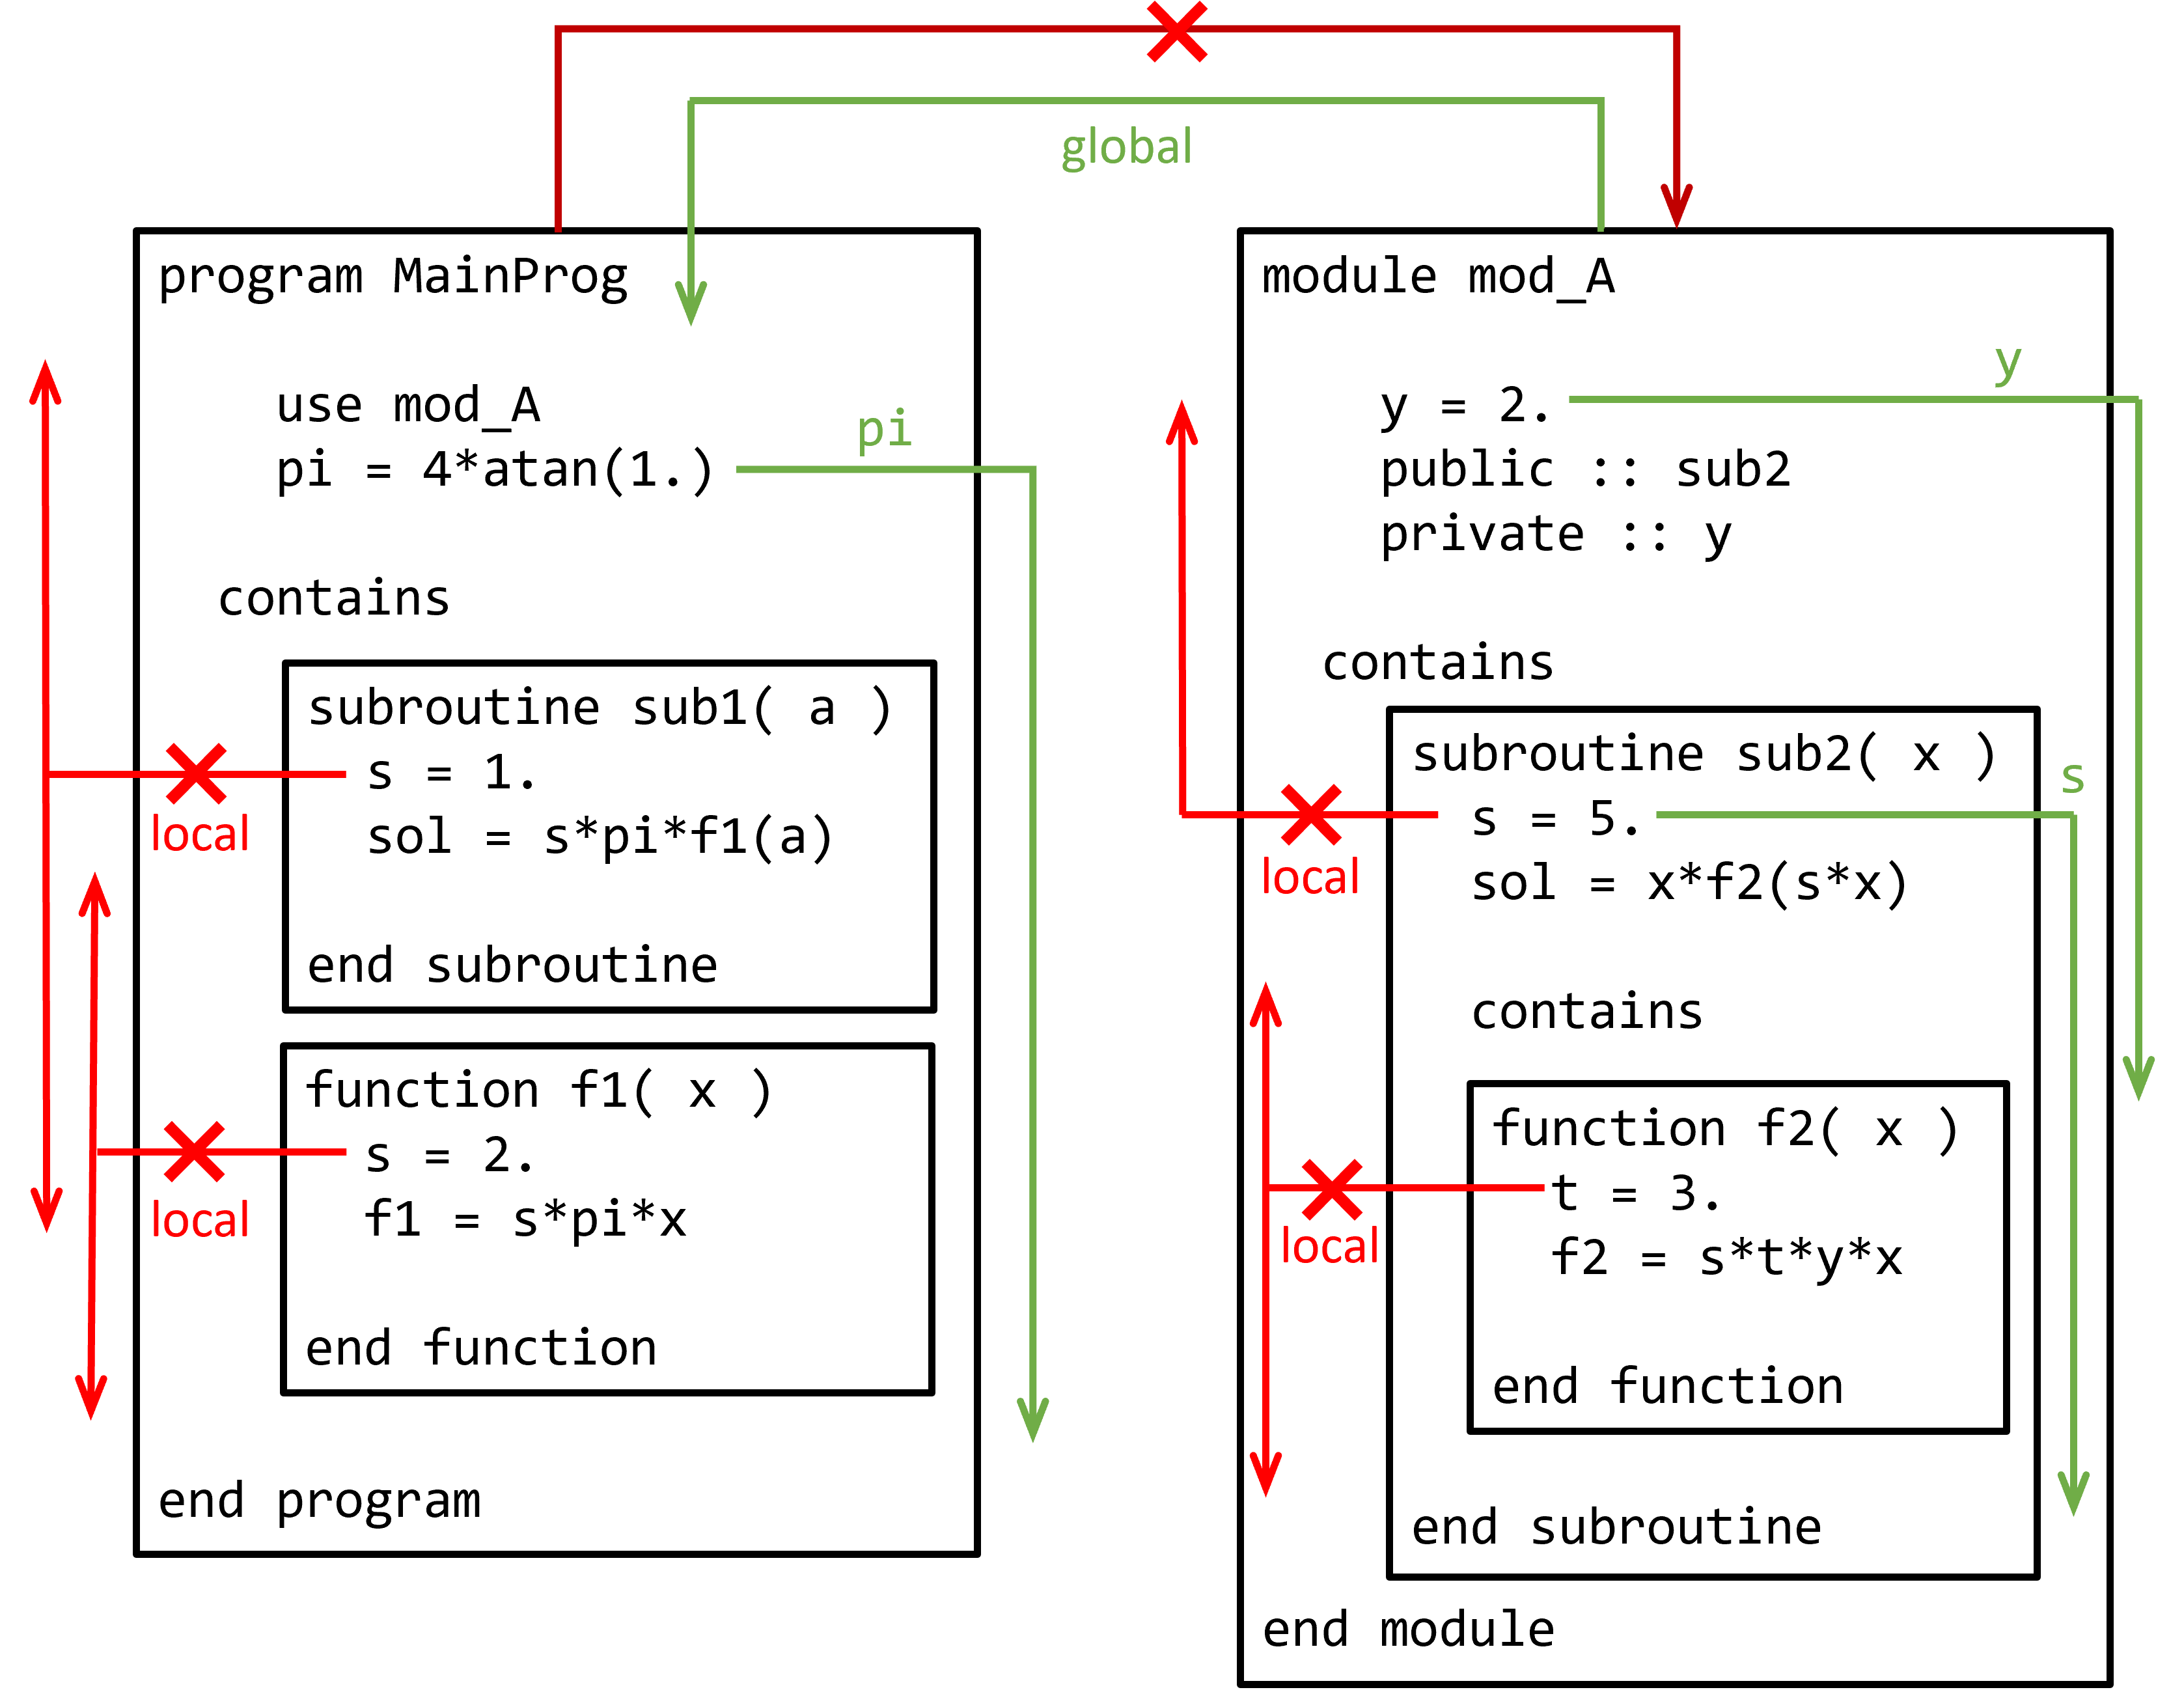
\includegraphics[width= \textwidth]{./doc/Figures/ScopeFor.png}
    \caption{Example of scope for different variables and constants in both program units in Fortran. Notice that \texttt{MainProg} sees all entities of \texttt{mod\_A} by default, however, since \texttt{y} is declared as private, it won't be seen. Furthermore, function \texttt{f2( x )} is only accessible inside the subroutine \texttt{sub2( x )}, it won't be accessible from anywhere else. Finally, notice that \texttt{sub1( a )} sees \texttt{f1( x )} since both are global in the main program.}
    \label{fig:ScopeFor}
\end{figure}


Python also works with a main application and external modules defined in different files. 
Each variable, object, function, etc. is treated in the following way (see Figure \ref{fig:ScopePy}):
\begin{itemize}
    \item Everything declared in the main body of the Python code will be treated as global. 
    Hence, this entity is seen throughout all the program whether is a function or not.
    
    \item On the contrary, entities declared inside functions are local and its scope is limited to the function itself. 
    More specifically, a function nested in another function sees the local variables declared in the host function.
    
    \item If a local variable uses the same name as a global variable, Python will separate them as two, one accessible from the global scope and other accessible from the local scope. 
    The function by default won't be able to access or modify the value of the global entity.
    Then, the attribute \texttt{global} can be used to ensure that the name of the variable refers to the global entity inside the function.
    
    \item To make functions, variables, etc. declared in modules visible in the main application the \texttt{import} statement is used. 
    Notice that then the module is called before the specific function: \texttt{module.function()}.
    To import only a part of the module, for example a function, the notation \texttt{from <module> import <name>} is used. 
    Then, the specific \texttt{<name>} can be called directly in the code with no need of calling first the module.
\end{itemize}

\begin{figure}[h]
    \centering
    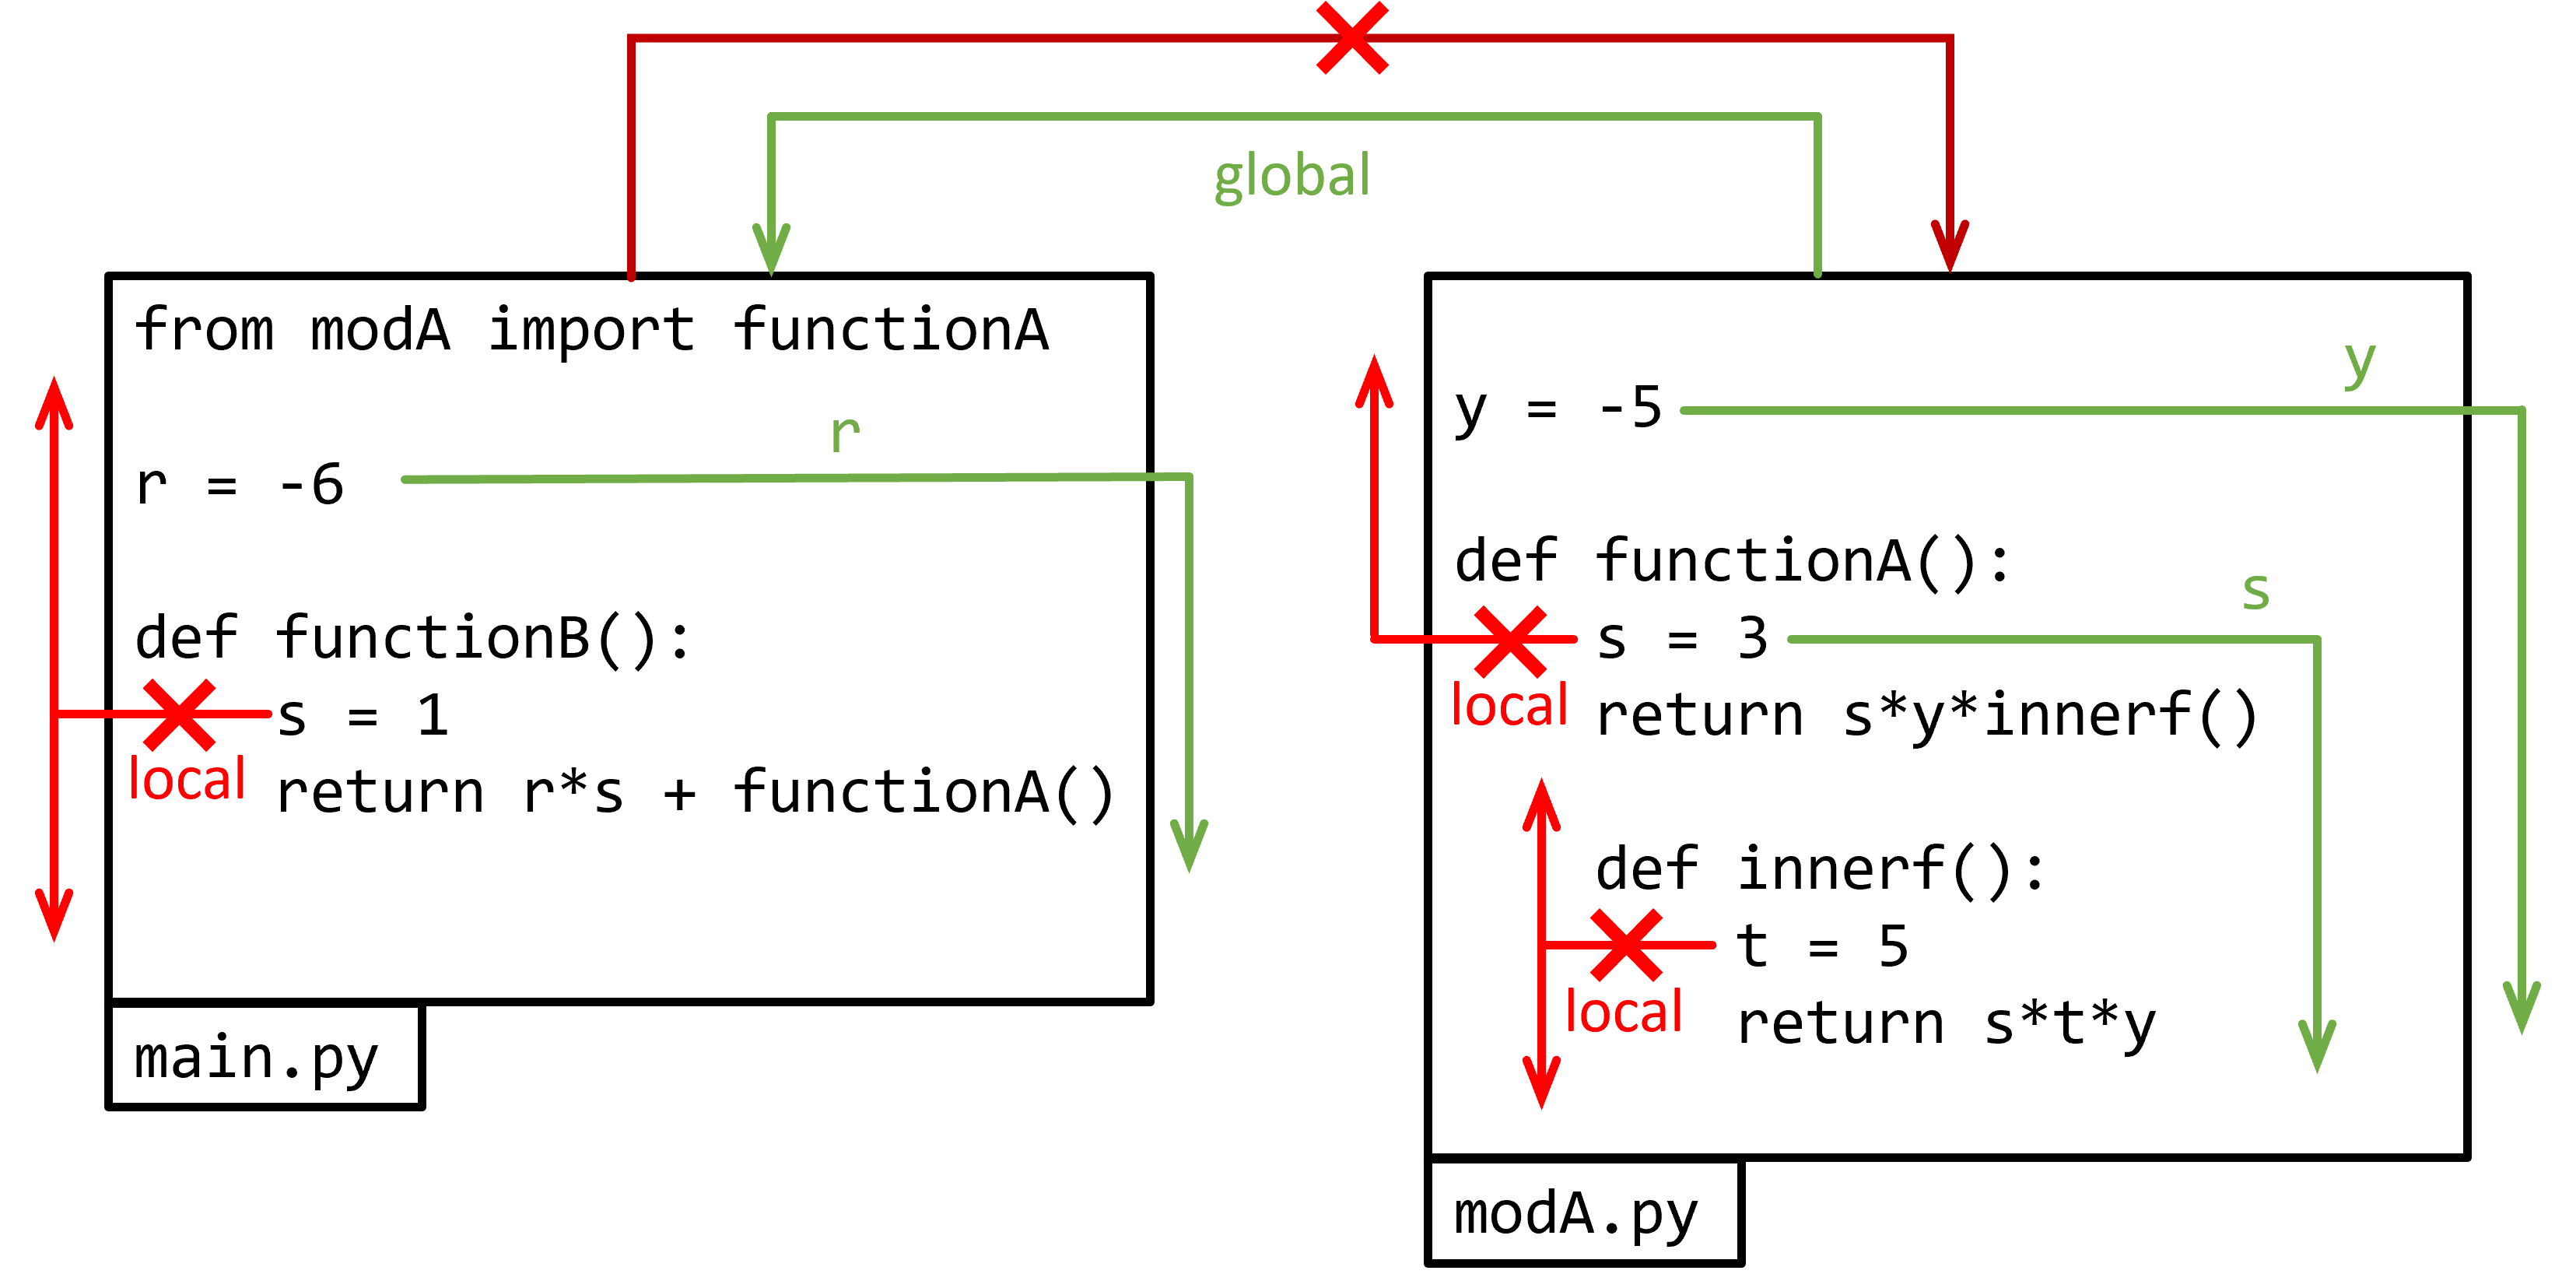
\includegraphics[width= \textwidth]{./doc/Figures/ScopePy.png}
    \caption{Example of scope for different variables and constants in the main application and a module in Python. Notice \texttt{Main.py} sees only \texttt{f2( x )} from \texttt{modA.py} due to the selective import. In addition, function \texttt{innerf2( x )} is only accessible inside \texttt{f2( x )}, it won't be accessible from anywhere else.}
    \label{fig:ScopePy}
\end{figure}



\begin{IN}
    \begin{itemize}
        \item Reduce the scope of variables and other entities as much as possible to avoid name collision or incorrect use of global entities. 
        A function for example should get all the information needed from local variables and input arguments, thereby ensuring its result does not depend on external pieces of code.
        
        \item If a global variable is needed, then consider the use of \texttt{parameter} in Fortran so its value is protected from being changed throughout the code. 
        
        \item Using functions to modify the values of global variables (using \texttt{global} attribute in Python for example) is not recommended. 
    \end{itemize}    
\end{IN}









%In the following code,  variables $x, y,z $ are visible inside the subroutine \texttt{Test}.  
In the following code, the variable $y$ is a global variable of module \texttt{modB} and $x$ is a global variable of module \texttt{modA}.  
Then, $y$ is seen inside function \texttt{functionB()} and $x$ is seen in \texttt{functionA}.
All global variables of \texttt{modB} are seen outside by means of the sentence \texttt{use modB}. 
Besides, since \texttt{modB} uses \texttt{modA}, all global variables of \texttt{modA} are seen in \texttt{modB}. 
More specifically, this means that $x$ is also seen in \texttt{functionB()}. 
\vspace{0.5cm} 






\newpage  
\section*{Fortran}

\renewcommand{\home}{./Fortran/sources/Advanced_programming/scope} 

\lstfor
\listings{\home/modB.f90}{module modB}{end module}{modB.f90}

\listings{\home/modA.f90}{module modA}{end module}{modA.f90}


\newpage
\section*{Python}

\renewcommand{\home}{./Python/sources/Advanced_programming/scope} 

\lstpython
\listings{\home/modB.py}{from}{return}{modB.py}

\listings{\home/modA.py}{x}{return}{modA.py}





%The region of a program in which this variable or identifier is visible is called the scope.
%set of statements in which the variable can be used or modified
% This is called the scope of the visibility of some variable in some part of our code. 
%Local variables are those which specified inside the function or subroutine that we are dealing with and global variables are those that can be accessed by common variables of my own module  or by inclusions of other modules. 